\hypertarget{result-ii-quantum-mechanics-general-relativity-as-a-common-refinement-a-unification}{%
\section{Result II --- conditional QM--GR access structures and graph duality}\label{result-ii-quantum-mechanics-general-relativity-as-a-common-refinement-a-unification}}

\hypertarget{locating-the-obstruction-the-route-mismatch}{%
\subsection{Route mismatch: an exact commutation result}\label{locating-the-obstruction-the-route-mismatch}}

For idempotent endomorphisms \(E_1,E_2\), the finite defect
\[
\Delta_3^{\mathrm{comp}}(E_1,E_2)=\{c:E_1E_2(c)\ne E_2E_1(c)\}
\]
is a legitimate mathematical measure of non-commutation, and non-commuting examples exist. The natural QM--GR
instantiation, however, gives a null verdict. On the 16-state Boolean carrier, the two conditional-mean completions are
idempotent and \textbf{commute exactly}: \(E_{\rm QM}E_{\rm GR}=E_{\rm GR}E_{\rm QM}\), so the defect set is empty. A
naive normalized distance between the two encoded tables (\(0.5\); \(1/\sqrt2\) under \(0/1\to\pm1\) recoding) is
encoding-dependent and is not a conjugacy-invariant commutator magnitude.

Coordinate conditional means commute here because the Boolean-cube overlap factorizes. Non-commuting idempotent pairs
can be constructed from non-factorizing partitions and constrained projections as mathematical controls,
but none is derived from the frozen ``quantize'' and ``curve'' routes. No route-mismatch explanation of why
quantizing gravity fails is therefore available at this level. Exact matrices and recoding controls are in
\nolinkurl{review_2026/repairs/q2_route_mismatch/}.

\hypertarget{the-resolution-a-fork-not-a-ladder}{%
\subsection{Fork-over-ladder, with finite provenance}\label{the-resolution-a-fork-not-a-ladder}}

A separate access-factorization result holds, narrowly. On the abstract four-coordinate carrier
\[
q_{\rm QM}=(d_0,d_1,d_2),\qquad q_{\rm GR}=(d_0,d_2,d_3),\qquad L=(d_0,d_1,d_2,d_3),
\]
\(q_{\rm GR}\) is not a deterministic quotient of \(q_{\rm QM}\): the two directed defects each have eight witnesses.
The nested coordinate control factors, while both readouts factor through \(L\) by definition. Exhausting all 16
coordinate-subset partitions gives 55 incomparable pairs among the 120 unordered distinct pairs. This is an exact toy
theorem conditional on the abstract carrier and its access interpretation; it is consistent with, and does not
contradict, the exact commutation of §5.1.

A finite provenance construction replaces bare mode labels. On 54
constructed \((\psi,V_0)\) records, coarse field functionals and explicit phase-only and potential controls realize
mutually non-factorizing QM and GR readouts. Its conditions are material: the forward witness changes \(V_0\), the QM
audit includes density and current rather than Born density alone, \(d_0\) is constant, and the realized coordinate
image is \(1\times2\times8\times3\), not the full \(2^4\) carrier. Nine hand-instantiated F24 representatives were
tested; two reconcile but are partition-equivalent to \(L\). Thus this is \textbf{conditional finite provenance}, not
family, type, or instance uniqueness. See \nolinkurl{review_2026/repairs/q1_access_provenance/}.

The theorem named \(T_{\mathrm{QG\text{-}NoGo}}\) is narrow: it tests two special fused or
stapled routes and does not quantify over general fused objects, coherent mediators, or operator algebras. It cannot
support any statement that quantum gravity is ``illegal'' in the grammar.

\begin{figure}[tbp]
  \centering
  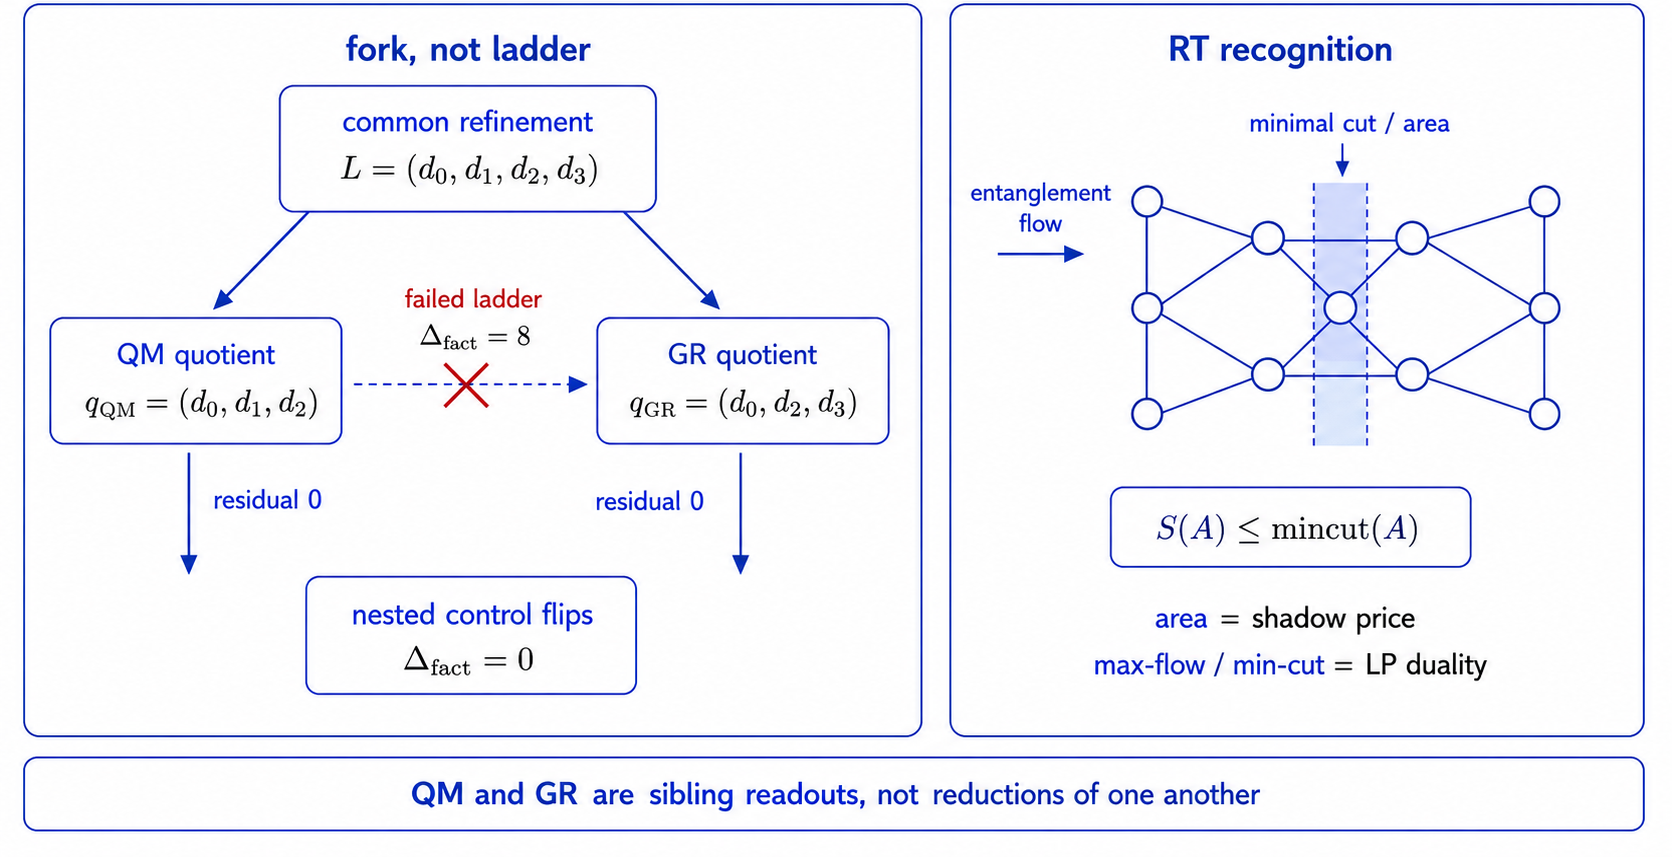
\includegraphics[width=\linewidth]{figures/fig_f3_fork_rt.png}
  \caption{\textbf{Finite fork and graph-duality constructions.} Left: the declared abstract access fork, for which the
  directed quotient fails and the common refinement closes. Right: a boundary-anchored flow network; the
  identity distinguishes the dual optimum from its per-edge shadow prices.}
  \label{fig:f3}
\end{figure}

\hypertarget{grounding-the-premise}{%
\subsection{The common carrier is a hypothesis}\label{grounding-the-premise}}

The common-carrier premise is not computationally grounded by the available tests. Semiclassical co-sourcing---one field
\(\psi\) supplying a Born-type readout and stress-energy for a potential---is a plausible named recognition source,
but the existing controls test different predicates and the ``door test'' is prose. The premise is therefore
carried as a declared hypothesis, not a GROUND landing. The 54-record construction above shows that a finite realization can
be built under explicit choices; it does not establish that nature, the free gravitational sector, or a deep
quantum-gravity regime shares such a carrier.

\hypertarget{recognition-ryutakayanagi-as-ledgershadow-price-duality}{%
\subsection{Finite-graph min-cut/LP-duality recognition}\label{recognition-ryutakayanagi-as-ledgershadow-price-duality}}

At nondegenerate seeded capacities, every tested
boundary region has a unique minimum cut with an exported margin. The max-flow primal and cut dual are exported as
matrices, and exact certificates verify strong duality and complementary slackness. If \(y_e\) denotes the dual
variable associated with edge capacity \(c_e\), then the identity is
\[
\operatorname{Area}(\operatorname{mincut}A)
=\operatorname{OPT}_{\rm dual}(A)
=\sum_e c_e y_e,
\]
where the \(y_e\)---not the dual optimum---are per-edge shadow prices. In the unique-cut chamber they are the \(0/1\)
cut-incidence variables and satisfy \(y_e=\partial F^*/\partial c_e\), verified by two-sided perturbations.

Independently contracted random-tensor states obey \(S(A)\le\operatorname{mincut}(A)\) on the sampled carrier. The ratios
\(S/\operatorname{mincut}=0.729,0.904,0.941\) for bond dimensions \(D=2,3,4\) are a \emph{finite sampled saturation
trend}, not convergence or equality; sampled contracted-state entropies remain below the cuts. The min-cut entropy
vectors satisfy monogamy, and a fairly compared GHZ control violates it. These results support a
\textbf{finite-graph recognition} of RT-related structure, conditional on the graph/tensor-network model; they do not
derive holography~\citep{RyuTakayanagi2006,Maldacena1998}, \(1/4G\), or a continuum law.

Two natural extensions fail, and the failures are results in their own right. First, there is no linearized-Einstein
match: a pass can be manufactured at a degenerate point, but
at an honest nondegenerate base point an independently specified geometry deformation does not match the
contracted-state \(\delta S\) under the declared pairing; uniqueness margins and a can-fail deformation are exported.
Second, Born and area do not carry one universal composition law: area follows min-plus composition on all four tested
gluing probes, while Born fails all four. The cross-ledger statement is only that the two sampled ledgers
obey the same monogamy inequality class, with different dependencies. See
\nolinkurl{review_2026/repairs/q5_lp_duality/}.

\hypertarget{result-qmgr-summary-table}{%
\subsection{Certified summary}\label{result-qmgr-summary-table}}

\begin{longtable}[]{@{}p{0.28\linewidth}p{0.22\linewidth}p{0.42\linewidth}@{}}
\toprule
question & status & certified scope\\
\midrule
\endhead
route mismatch & exact null result & completions commute; \(0.5\) is encoding-dependent table distance\\
fork-over-ladder & narrow exact theorem & exact coordinate-partition non-factorization on the declared Boolean carrier\\
field provenance & conditional finite construction & 54 records with named coarse functionals and stated limitations\\
common-carrier premise & hypothesis & semiclassical co-sourcing is a named physical motivation, not a landing\\
\(T_{\mathrm{QG\text{-}NoGo}}\) & narrow & two special fused/stapled routes only\\
RT/LP relation & finite-graph recognition & exact dual certificate and sensitivities on finite nondegenerate graph cuts\\
linearized Einstein & negative result & tested response does not match under the declared deformation pairing\\
one Born--area ledger & negative result & area passes four min-plus gluings; Born fails all four\\
\bottomrule
\end{longtable}
